\chapter{XJ: Graphics Programming for XSB}

Graphical system software for XSB is based on two systems: the
open-source InterProlog \cite{Cale01}~\footnote{InterProlog is
available through \url{www.declarativa.com}.}, and the XJ system,
which is proprietary to XSB, Inc.  While a full description of these
systems is beyond the scope of this paper, we overview some of their
important features here.

\section{InterProlog}

The InterProlog system provides a mechanism for XSB and Java to
intercommunicate at a finely-grained level.  Using InterProlog, a Java
message can be invoked via the predicate {\tt javaMessage} (of various
arities); and an XSB goal can be invoked via various Java messages.
From Java's point of view, Prolog is modeled by the Java class {\tt
PrologEngine}.  The extension {\tt SubprocessEngine} provides
mechanisms for XSB and Java to communicate through sockets; the
extension {\tt NativeEngine} allows XSB and Java to communicate
through Java's native interface, and it is this latter communication
that the CDF editor uses.  In either case InterProlog maps a Java
object to a Prolog term.  When a Java object is sent to Prolog {\sc
through ???}, Java's object serialization protocol is used to
translate the object to a stream of bytes.  This stream is read by
Prolog and parsed using a definite clause grammar.  When a Prolog term
is sent to Java, a definite clause grammar is again used to generate a
stream of bytes that will be read by Java.

\section{XJ}

\subsection{Prolog Types}

termSetGui; tree, table.

\subsection{XJ Types}

xjtree ; xjtable ; xjcomponent; Jcomponent.

\subsection{xjdisplays}

ParWin ; Title

Mention that not all features are documented.

\begin{description}

\xjitem{chooseFromTerms(+Pred/Arity,+Type,+ContextDescription,+Context,+MaxChoices,-Picked)}{chooseFromTerms/6}
%\xjitem{chooseFromTerms(+TreeOrListGt,+MaxChoices,-Picked)}{chooseFromTerms/3}
%
Creates a \xjdom{termSetGui} term from {\tt Pred/Arity}, {\tt Type},
{\tt ContextDescription}, and {\tt Context}.  This term is then sent
as a parameter to an XJ class~\footnote{The
\xjclass{TermChooseDialog} class that extends \jclass{JDialog}.} that
allows one or more terms to be selected from the term set, returning
them in the list {\tt Picked}.  Currently, the term set must either be
an instance of \xjclass{XJTree} or \xjclass{XJTable}.  If the user
cancels the selection, an empty list is returned.  {\tt MaxChoices}
determines how many terms may be selected (chosen) by the user; 2 or
more means unbounded.  An example of a call to
\pred{chooseFromTerms/6} is shown in Figure~\ref{fig:chooseFromTerms}.

%-------------------------
\begin{figure}[htbp] \label{fig:chooseFromTerms}
\centering {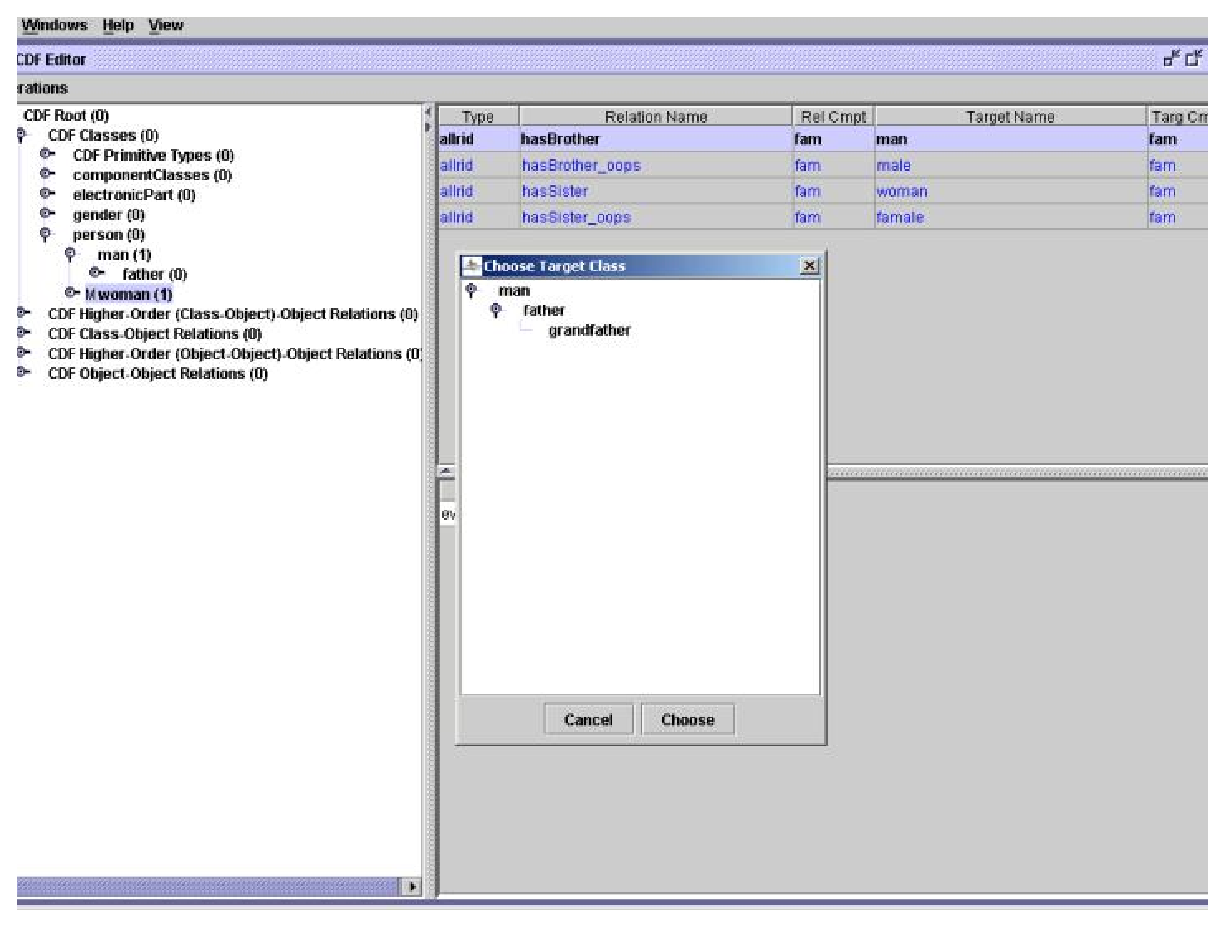
\epsfig{file=Figures/chooseFromTerms.eps,width=\textwidth}}
\caption{An example of {\tt chooseFromTerms/6} based on a term set of type {\tt XJTree}.}
\end{figure}
%-------------------------

%-------------------------------------------------------------------------------------------
\xjitem{xjConfirmUser(+ParWin, +Title, +Message)}{xjConfirmUser/3}
%
Creates a window \footnote{A \jclass{JOptionPane} of type
{\tt Confirm Dialog}.} allowing a user to confirm or cancel an
operation.  An example is shown in Figure~\ref{fig:xjConfirmUser}.

%-------------------------
\begin{figure}[htbp] \label{fig:xjConfirmUser}
\centering {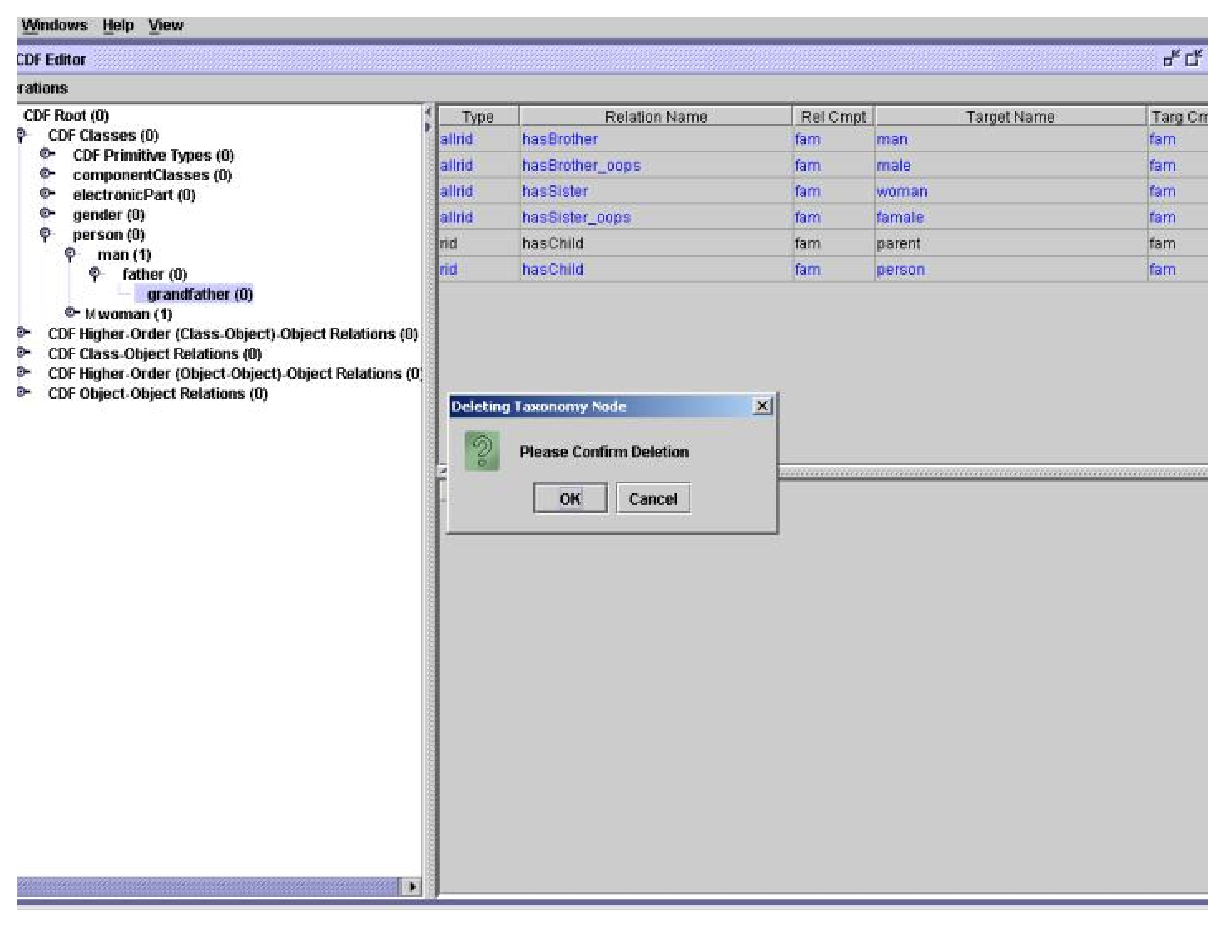
\epsfig{file=Figures/xjConfirmUser.eps,width=\textwidth}}
\caption{An example of xjConfirmUser}
\end{figure}
%-------------------------

%-------------------------------------------------------------------------------------------
%\xjrptitem{xjAskUser(+ParWin,+Question,?DefaultAnswer,-Answer)}{xjAskUser/5}
%
\xjitem{xjAskUser(+ParWin,+Title,+Question,?DefaultAnswer,-Answer)}
	{xjAskUser/5}
%
Creates a window \footnote{A \jclass{JOptionPane} of type {\tt Input
Dialog}.} allowing a user to input data and confirm or cancel that
data once it is input.
%-------------------------------------------------------------------------------------------

\xjitem{xjReportError(+ParWin,+Title,+Message)}{xjReportError/3}
Creates a window \footnote{A \jclass{JOptionPane} of type {\tt
Error Message Dialog} with an error icon.} informing a user of an error
condition specified by {\tt Message}.

\xjitem{xjNotifyUser(+ParWin,+Title,+Message)}{xjNotifyUser/3}
Creates a window \footnote{A \jclass{JOptionPane} of type {\tt
Inform Message Dialog} with a  icon.} notifying the user of an event
or condition specified by {\tt Message}.

%-------------------------------------------------------------------------------------------
%\xjitem{xjAskNumber(+ParWin,+Question,+Title,?InitialValue,+Type,-num(Result))} {xjAskNumber/5}
%
%Produces a modal dialog window  asking the user for a number.  Type can be
%the atom float or the atom Integer.

%-------------------------------------------------------------------------------------------

% Just a generic message.
%\xjitem{xjShowAboutDialog(+ParWin, +Title, +Message, +IconLocation)}
%{xjShowAboutDialog/4}
%Displays generic about dialog. 

%-------------------------------------------------------------------------------------------

% TLS ParWin in different place in the code.
\xjitem{xjShowOptionDialog(+ParWin,+Title,+Message,+ButtonList,-ButtonChosen)} {xjShowAboutDialog/5}
%
Display a modal dialog window \footnote{A \jclass{JOptionPane} of type
{\tt Question Message Dialog}.} with a question message and a set of
buttons to click on to answer that message.  An example is shown in
Figure~\ref{fig:xjShowOptionDialog}.

%-------------------------
\begin{figure}[htbp] \label{fig:xjShowOptionDialog}
\centering {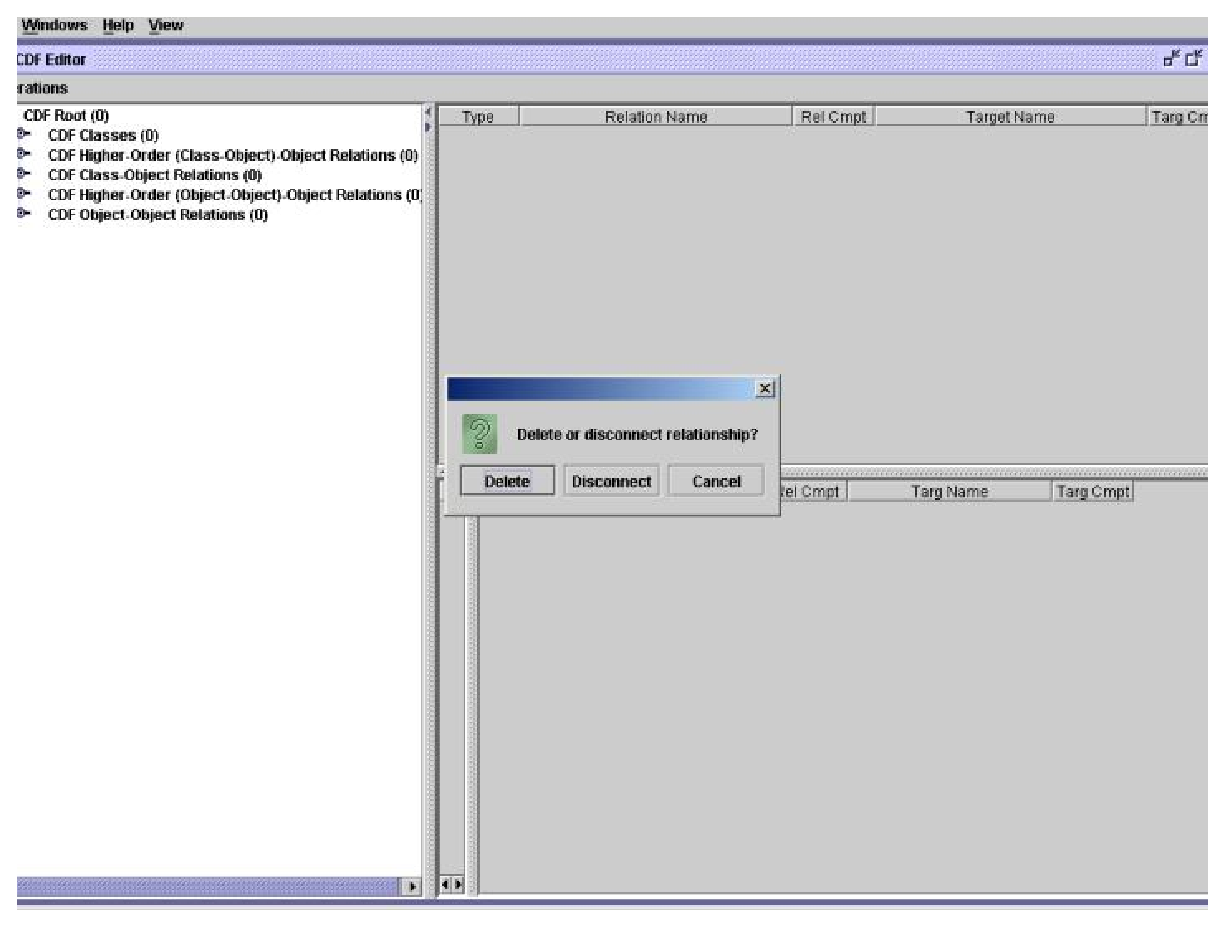
\epsfig{file=Figures/xjShowOptionDialog.eps,width=\textwidth}}
\caption{An example of xjShowOptionDialog}
\end{figure}
%-------------------------

%-------------------------------------------------------------------------------------------

\xjitem{xjPickFile(+Parent,+StartDir,+ExtensionList,+ApproveText,-File)
	}{xjPickFile/5}	
%
%\xjrptitem{xjPickFile(+StartDir,+ExtensionList,+ApproveText,-File)}{xjPickFile/4}
%
%\xjitem{xjPickFile(+ExtensionList,+ApproveText,-File)}{xjPickFile/3}
%
This predicate displays a Swing file chooser, and fails if the user
cancels the choice.  {\tt StartDir} is an atom signifying the starting
directory for the chooser, {\tt ApproveTest} is an atom , and {\tt
ExtensionList} is a list of atoms containing all file types that
should be shown without dot, e.g.  ['P',java].  {\tt xjPickFile/3}
uses the user home directory as the starting directory. {\tt ???
Parent}.

%--------------
\begin{figure}[htbp] \label{fig:xjPickFile}
\centering {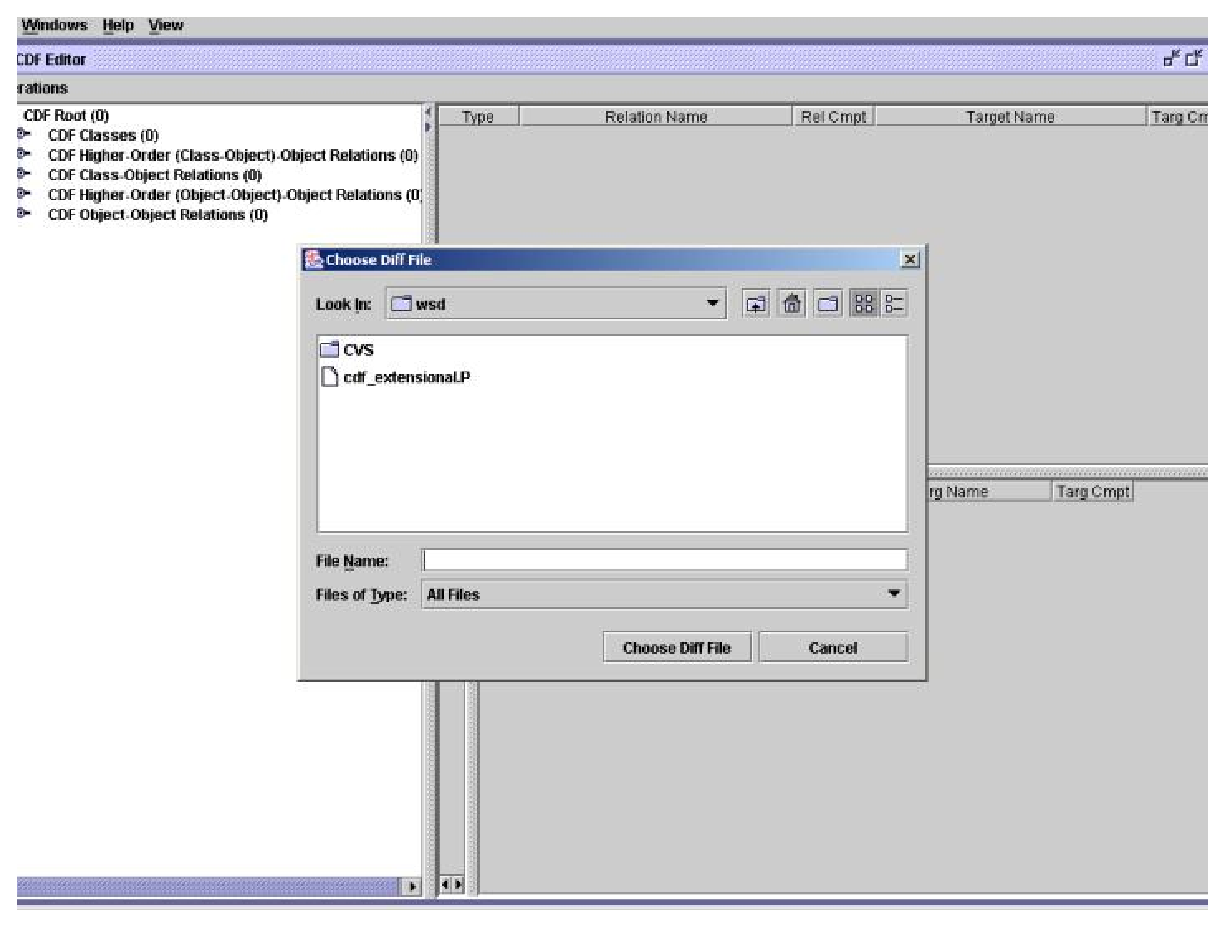
\epsfig{file=Figures/xjPickFile.eps,width=\textwidth}}
\caption{An example of xjPickFile}
\end{figure}
%--------------

\xjitem{xjPickDirectory(+Parent,+StartDir,+ApproveText,-Dir)}{xjPickDirectory/4}
%\xjrptitem{xjPickDirectory(+StartDir,+ApproveText,-File)}{xjPickDirectory/3}
%\xjitem{xjPickDirectory(+ApproveText,-File)}{xjPickDirectory/2}
%
This predicate displays a Swing file chooser, and fails if the user
cancels the choice.  For this predicate, only directories will be
displayed and chosen.  {\tt StartDir} is an atom signifying the
starting directory for the chooser, {\tt ApproveTest} is an atom.
{\tt xjPickDirectory/2} uses the user home directory as the starting
directory. {\tt ???  Parent}.

%-------------------------------------------------------------------------------------------

%\xjitem{xjShowURL(+URL)}{xjShowURL/1}
%Displays URL using system browser.

%\xjitem{xjViewDocument(+Location,+Viewer)}{xjViewDocument/2}
%Allows the use of the system viewer.

%-------------------------------------------------------------------------------------------

% Check out xj_display_errors, editTermGetResult
\end{description}

\subsection{Tree Templates}
	Generic class tree.

\subsection{Toolbar Widgets}
%    createNewMenu('Open',OPMenu),
%    addMenuItem(OPMenu, 'Project ...', open_project_commit),
%    addSubMenu(FileMenu,OPMenu),

